
Der erste Teilversuch befasst sich mit sogenannten dichroitischen Spiegeln. Diese sind dünne Platten, welche in optischen Anwendungen zur Aufspaltung und Filterung von bestimmten Wellenlängen des Lichts dienen. Erreicht wird dies durch Dünnfilminterferenz, welche Wellenlängen reflektiert bzw. unbeeinflusst durch den Spiegel passieren lässt. Für den später betrachteten LCD-Beamer filtern diese Spiegel die verschiedenen Farben aus der Lichtquelle, und sind so integraler Bestandteil dessen Farbwiedergabe.

Es sollen zwei dieser Spiegel von den Teilnehmenden mithilfe eines Spektrometers untersucht werden, um deren Transmissionsspektren zu messen. Darauffolgend können die Reflektionsspektren der Spiegel bestimmt werden, um somit die Farbpositionen der reflektierten Lichtstrahlen im Farbdreieck zu bestimmen.

\subsubsection{Versuchsaufbau} Dieser besteht aus einer möglichst weißen, gleichmäßig über das sichtbare Spektrum strahlenden Lichtquelle, hier einer blauen LED mit gelben Phosphoren. Das Licht der LED wird mithilfe einer Linse zu einem Strahl gebündelt, welcher auf die Messapertur eines Spektrometers gerichtet wird. Das Spektrometer ist von einem Computer aus bedienbar und die vom Spektrometer aufgenommenen Messungen können gespeichert werden. Zusätzlich steht den Teilnehmenden eine Halterung zur Verfügung, mit derer sich die dichroitischen Spiegel in den Lichtstrahl der LED, vor dem Spektrometer, in einem $45^\circ$-Winkel relativ zum Lichtstrahl befestigen lassen. Dies ist der Winkel für welchen die Spiegel optimiert wurden. Das reflektierte Licht wird auf eine weiße Abschirmung gespiegelt, um sichtbar gemacht zu werden. Ein schematischer Versuchsaufbau ist in Abbildung \ref{abb:V1_AUFBAU} zu sehen. Dort ist links die Lichtquelle mit fokussierender Linse, die zwei schwarzen Streifen stellen die dichroitischen Spiegel dar, und das Spektrometer misst das nach rechts geleitete Licht.

\begin{figure}[h]
	\centering
	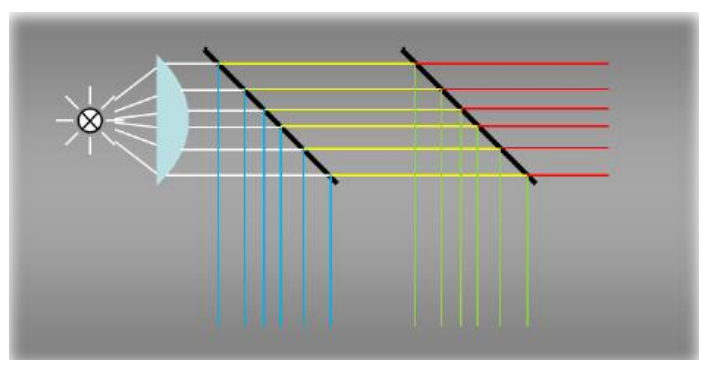
\includegraphics[scale=0.4]{Images/Aufbau.png}
	\caption{Schematischer Versuchsaufbau, [\cite[Abb. 3.2]{AML_SKRIPT}]}
	\label{abb:V1_AUFBAU}
\end{figure}

\newpage
\subsubsection{Versuchsdurchführung}

Die Messung der Transmissionsspektren der Spiegel erfolgt in vier Schritten:
\begin{itemize}
\item Bestimmung einer Integrationszeit, bei welcher das Spektrometer zu etwa 90\%, nie aber 100\% belichtet wird. Hierdurch wird eine Überbelichtung und somit Verfälschung der Messergebnisse verhindert. Im Folgenden wird eine Integrationszeit von 90ms gewählt.
\item Durchführung einer Dunkelmessung des Hintergrundlichtes, um dieses aus den Messwerten entfernen zu können.
\item Durchführung einer Referenzmessung (100\%-Messung) der LED ohne eingebaute Spiegel. Mit dieser werden die späteren Messwerte automatisch in Relation gesetzt, um somit die relativen Anteile des transmittierten Lichtes berechnen zu können.
\item Messung der transmittierten relativen Spektren bei eingebauten Spiegeln 1 bzw. 1+2
\end{itemize}
In der folgenden Grafik sind die drei relevanten Kurven der relativen Spektren von Referenzmessung, von Spiegel 1 und von Spiegel 1+2 im sichtbaren Frequenzbereich dargestellt:

\begin{figure}[h]
	\centering
	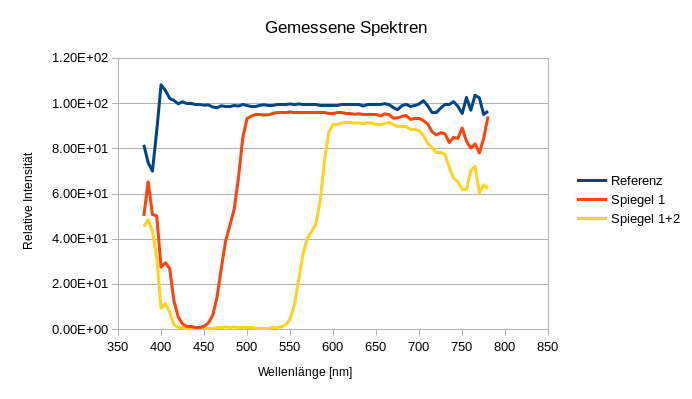
\includegraphics[scale=0.8]{Images/V1_Spektren.png}
	\caption{Relative Spektren der Spiegel im Vergleich}
	\label{V1_RES}
\end{figure}

\subsubsection{Auswertung}

\label{V1_AUSW}

Zuerst wird die Kurve der Referenzmessung (relativ zu den gemessenen Referenzwerten) betrachtet. Überwiegend liegt diese bei 100\%, wie es von der Referenzmessung zu erwarten ist. An der oberen und unteren Grenze des für den menschlich sichtbaren Wellenlängenbereiches kommt es jedoch zu Schwankungen. Diese lassen sich dadurch erklären, dass die verwendete LED in diesen Wellenlängen sehr schwach bis nicht leuchtet, und die Messwerte hierdurch stark vom Hintergrundrauschen beeinflusst werden. 

Das Spektrum des ersten Spiegels in Abb. \ref{V1_RES} lässt nun auf zweierlei schließen:
Der Spiegel transmittiert nie zu 100\%, es wird anscheinend immer ein kleiner Teil des Lichtes reflektiert bzw. absorbiert. Erkennbar ist dies daran, dass die Kurve nie ganz 100\% erreicht. Zweitens ist deutlich der Bereich der Reflekion zwischen 400nm und 500nm zu erkennen, in welchem der Spiegel fast 100\% des Lichtes reflektiert. 

Schließlich wird das Spektrum beider Spiegel (1+2) betrachtet. Erstens ist zu erkennen, dass es im Vergleich zu Spiegel 1 eine stärkere allgemeine Reflektion bzw. Absorption auch in nicht-reflektierten Wellenlängen gibt. Zweitens ist zu erkennen, dass der zweite Spiegel einen Wellenlängenbereich von ca. 450nm bis 600nm reflektiert, da dort keines des vom Spiegel 1 durchgelassenen Lichtes mehr am Sensor an kommt.

Nun werden die jeweiligen relativen reflektierten Spektren der Spiegel, sowie das von beiden Spiegeln transmittierte Spektrum, ermittelt.
Im Folgenden gilt die Annahme, dass die Spiegel das gesamte Licht entweder reflektieren oder transmittieren.
Für das vom ersten Spiegel reflektierte Licht wird von der relativen Referenzmessung ($D_{\lambda,0}$) das relative Transmissionsspektrum des ersten Spiegels ($D_{\lambda,1}$) abgezogen.
Für das am zweiten Spiegel reflektierte relative Spektrum wird vom transmittierten Spektrum des ersten Spiegels das transmittierte Spektrum des zweiten Spiegels ($D_{\lambda,2}$) abgezogen. Es gelten folgende Gleichungen:
\begin{eqnarray*}
	T_{\lambda, 1}(\lambda) = & D_{\lambda,0}(\lambda) - D_{\lambda,1}(\lambda) \\
	T_{\lambda, 2}(\lambda) = & D_{\lambda,1}(\lambda) - D_{\lambda,2}(\lambda) \\
	T_{\lambda, 3}(\lambda) = & D_{\lambda,3}(\lambda)
\end{eqnarray*}
Es ergeben sich folgende Kurven:

\begin{figure}[h]
	\centering
	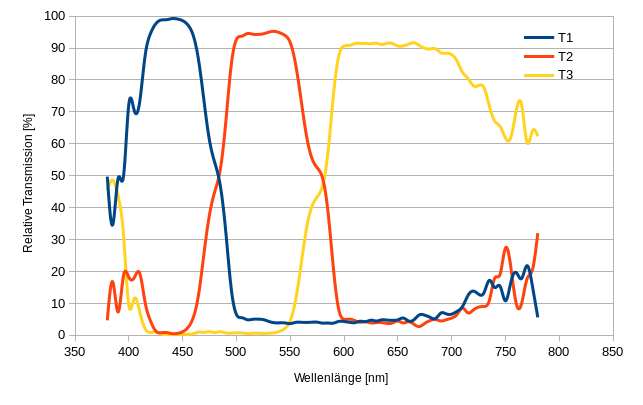
\includegraphics[scale=0.8]{Images/V1_Transmissionen.png}
	\caption{Berechnete relative Transmissionsspektren der aufgespalteten Strahlen}
	\label{V1_REFLECT}
\end{figure}

Die vorher vermuteten Reflektionsbereiche von 400nm bis 500nm bzw. 450nm bis 600nm sind hier gut erkennbar. Die Schwankungen des Reflektionsspektrums der Spiegel unter 450nm und über 730nm lassen sich durch niedrige absolute Werte erklären, welche somit stärker rauschen.
Das Verhalten der Spiegel kann somit als Bandsperrfilter angenähert werden, welche für die obig genannten Wellenlängenbereiche das Licht reflektieren, ansonsten beinahe ungestört transmittieren.